\documentclass[11pt,a4paper]{article}
\usepackage{tikz}
\usetikzlibrary{angles,quotes}

\usepackage{amsmath}
\usepackage{amsfonts}
\usepackage{amssymb}
\usepackage{graphicx}
\usepackage[left=2cm,right=2cm,top=2cm,bottom=2cm]{geometry}
\usepackage{multicol}
\usepackage{float}
\restylefloat{table}

\newcommand\Base[1][0]{
\begin{scope}[xshift=#1]
\clip
  (-0.5,5.5) rectangle (5.5,-0.5);
  \draw[->]
  (-0.5,0) -- (5,0) node[right] {$u$};
\draw[->]
  (0,-0.5) -- (0,5) node[above] {$v$};
\coordinate (O) at (0,0) node[above left] {$O$};
\coordinate (aux1) at (40:4);
\coordinate (aux2) at (aux1|-0,0);
\coordinate (aux3) at (4,{4*tan(40)});
\node at (4.2, 0.2) {$A$};
\node at (3.1, 3) {$B$};
\node at (4.2, 3.7) {$C$};
\draw
  (O) -- (aux3) -- (aux3|-0,0)
  (aux1) -- (aux2);
\draw[thick,red!70!black] 
  (O) circle (4);
\pic[draw,"$x$",angle radius=30pt,angle eccentricity=1.2] {angle = aux2--O--aux1};   
\end{scope}  
}

\author{Iker M. Canut}
\title{Unidad 3: L\'imite y Continuidad\\ Analisis Matem\'atico I}

\newcommand*{\QEDA}{\null\nobreak\hfill\ensuremath{\blacksquare}}
\newcommand*{\QEDB}{\null\nobreak\hfill\ensuremath{\square}}

\begin{document}
\maketitle
\newpage

\section{Distancia de Puntos y Entornos}
Para $x,y \in \mathbb{R}$, la \textbf{distancia} entre $x$ e $y$ es $d(x,y) = |x-y|$\\

Llamamos \textbf{entorno} de un real $a$, de radio $\delta$ al intervalo abierto $(a-\delta, a+\delta)$ y lo notamos\\ $E(a,\delta) = \{x\in\mathbb{R}:a-\delta<x<a+\delta\} = \{x\in\mathbb{R}:-\delta<x-a<\delta\} = \{x\in\mathbb{R}:|x-a|<\delta\}$

Llamamos \textbf{entorno reducido} de un real $a$, de radio $\delta$ al conjunto $E(a,\delta) - \{a\}$ y lo notamos $E'(a,\delta) = \{x\in\mathbb{R}:|x-a<\delta\land x\not = a|\} = \{x\in\mathbb{R}:0<|x-a|<\delta\}$\\

Sea $a$ un real, $\delta_1, \delta_2$ dos reales positivos, y $\delta\leq min\{\delta_1, \delta_2\}$, se tiene que:
\begin{table}[h]
\centering
\begin{tabular}{ccc}
$E(a,\delta) \subseteq E(a,\delta_1) \cap E(a,\delta_2)$ & \ \ \ \ & $E'(a,\delta) \subseteq E'(a,\delta_1) \cap E'(a,\delta_2)$\\
$|x-a|<\delta \Rightarrow |x-a|<\delta_1 \land |x-a|<\delta_2 \hfill$ & \ y \ & $\hfill 0<|x-a|<\delta \Rightarrow 0<|x-a|<\delta_1 \land 0<|x-a|<\delta_2$
\end{tabular}
\end{table}

\section{L\'imite Finito en un Punto}
Dada una funci\'on real $f$ y un real $a$, tal que $f$ est\'a definida en un entorno reducido del punto $a$, decimos que $l$ es el l\'imite de la funci\'on $f$, cuando la variable independiente tiende al valor $a$ y notamos $$\lim_{x\to a}f(x)=l$$ si para cualquier valor $\epsilon > 0$, prefijado, existe un n\'umero positivo $\delta$ tal que: $$0<|x-a|<\delta \Rightarrow |f(x)-l| < \epsilon$$ $$x \in E'(a, \delta) \Rightarrow f(x) \in E(l, \epsilon)$$ $$\forall \epsilon > 0, \exists \delta > 0 /\ \forall x : (0 < |x-a| < \delta \Rightarrow |f(x)-l|<\epsilon)$$\\

No se exige que $a$ est\'e en el dominio de $f$, pero si que $f$ este definida en un entorno reducido de $a$.\\
La siguiente simbolog\'ia es equivalente:
\begin{table}[h]
\centering
\begin{tabular}{ccc}
$\displaystyle{\lim_{x\to a}f(x)=l}$ \ \ & \ \ $\displaystyle{\lim_{x\to 0}f(x+a)=l}$ \ \ & \ \ $\displaystyle{\lim_{x\to a}f(x) - l =0}$
\end{tabular}
\end{table}

Por \'ultimo, observamos que el n\'umero $\delta$ depende tanto del valor de $\epsilon$ como del punto $a$. Adem\'as, si en un punto $a$, para un $\epsilon$, un n\'umero $\delta$ satisface la definici\'on de l\'imite, entonces cualquier $\delta'<\delta$ tambien es v\'alido. Por otro lado, si un $\delta$ es \'util para un $\epsilon$, tambi\'en es \'util para un $\epsilon' > \epsilon$. $$0 < |x-a| < \delta' \Rightarrow 0 < |x-a| < \delta \Rightarrow |f(x)-l| < \epsilon < \epsilon'$$

\section{L\'imites Finitos}
\subsection{Funci\'on Constante}
$f(x)=c \in \mathbb{R}$, $\displaystyle{\lim_{x\to a}c=c}$, pues cualquier $\epsilon > 0$ y $\delta > 0$, se verifica que $$0<|x-a|<\delta \Rightarrow |f(x)-c| = |c-c| = 0 < \epsilon$$

\subsection{Funci\'on Lineal}
$f(x)=mx+h, m \not = 0$, $\displaystyle{\lim_{x\to a}mx+h=ma+h}$
$$\forall\epsilon>0,\ \exists\delta>0:\ \forall x: (0<|x-a|<\delta \Rightarrow |f(x)-l|<\epsilon)$$
$$|(mx+h)-(ma+h)| = |m|\cdot|x-a| < \epsilon \Rightarrow |x-a| < \delta < \dfrac{\epsilon}{|m|}$$
Y considerando $\delta < \dfrac{\epsilon}{|m|}$ tenemos que $0<|x-a|<\delta<\dfrac{\epsilon}{|m|} \Rightarrow |(mx+h)-(ma+h)|=|m|\cdot|x-a| < \epsilon$

\subsection{Funci\'on Cuadratica}
$f(x)=x^2$, $\displaystyle{\lim_{x\to a}x^2=a^2}$ hay que demostrar $\forall\epsilon>0,\ \exists\delta>0:\ \forall x: (0<|x-a|<\delta \Rightarrow |x^2-a^2|<\epsilon)$
Se ve que $|x^2-a^2| = |x-a|\cdot|x+a|$
\begin{itemize}
\item Caso $a=0$: $\forall\epsilon>0,\ \exists\delta>0:\ \forall x: (0<|x|<\delta \Rightarrow |x^2|<\epsilon)$\\
Luego $|x^2|<\epsilon \iff |x|^2<\epsilon \iff |x|<\sqrt{\epsilon}$ y tenemos que: $$0<|x|<\delta=\sqrt{\epsilon} \Rightarrow |x|^2<\epsilon \Rightarrow |x^2|<\epsilon$$
\item Caso $a\not = 0$: $\forall\epsilon>0,\ \exists\delta>0:\ \forall x: (0<|x-a|<\delta \Rightarrow |x-a|\cdot|x+a|<\epsilon)$ \hfill \textbf{(1)}\\
Hay que acotar $|x+a|$. Sea $0<\delta<|a|$, \hfill \textbf{(2)}
\begin{align*}
|x-a|<\delta &\Rightarrow -|a|<-\delta<x-a<\delta<|a| \Rightarrow -|a|+2a<-\delta+2a < x+a < \delta+2a < |a|+2a\\
& \Rightarrow -|a|-2|a| < x+a < |a|+2|a| \Rightarrow |x+a| < 3|a|
\end{align*}
Y tenemos que $|x-a|<\delta \Rightarrow |x+a| < 3|a|$. \hfill \textbf{(3)}\\
De \textbf{(2)} para que se verifique \textbf{(3)} y de \textbf{(1)} tenemos que $\delta\leq min\left\{|a|, \dfrac{\epsilon}{3|a|}\right\}$\\
Luego, $|x-a|<\dfrac{\epsilon}{3|a|} \land |x+a|<3|a|$. Y tenemos que $$0<|x-a|<\delta \Rightarrow |x^2-a^2| = |x-a|\cdot|x+a| < \dfrac{\epsilon}{3|a|}\cdot 3|a| = \epsilon$$
\end{itemize}

\subsection{Funci\'on Reciproca}
$f(x)=\dfrac{1}{x}$, $\displaystyle{\lim_{x\to a}\dfrac{1}{x}=\dfrac{1}{a}}$ hay que demostrar $\forall\epsilon>0,\ \exists\delta>0:\ \forall x: (0<|x-a|<\delta \Rightarrow |\dfrac{1}{x}-\dfrac{1}{a}|<\epsilon)$\\

\indent Se demuestra fijando un $\epsilon$ a cualquier n\'umero. Despu\'es se calcula la otra parte del m\'inimo.

\section{Unicidad del L\'imite}
\noindent \textbf{Teorema 1}: \textbf{Unicidad del L\'imite}. Sea $f$ una funci\'on real definida en un entorno reducido del punto $a$ y sean $l_1$ y $l_2$ dos n\'umeros reales tales que: \ \ $\displaystyle{\lim_{x\to a}f(x)=l_1} \ \land \ \displaystyle{\lim_{x\to a}f(x)=l_2} \ \ \Rightarrow \ \ \ \ l_1 = l_2$\\
\textbf{Demostraci\'on: } Dado $\epsilon > 0$, tenemos $\delta_1$ y $\delta_2$ tales que: $$0 < |x-a| < \delta_1 \Rightarrow |f(x) - l_1| < \dfrac{\epsilon}{2} \ \ \land \ \ 0 < |x-a| < \delta_2 \Rightarrow |f(x) - l_2| < \dfrac{\epsilon}{2}$$
Considerando $\delta = \min\{\delta_1, \delta_2\}$, considerando cualquier $E'(a, \delta)$, tenemos que:
$$|l_1 - l_2| = |l_1 - f(x) + f(x) - l_2| \leq |l_1 - f(x)| + |l_2 - f(x)| < \dfrac{\epsilon}{2} + \dfrac{\epsilon}{2} = \epsilon$$
Y como tenemos $0 \leq |l_1 - l_2| < \epsilon$, podemos asegurar que $|l_1 - l_2| = 0 \Rightarrow l_1 = l_2$ \QEDA

\section{No Existencia de L\'imite}
Negando la forma proposicional de la definici\'on de l\'imite, llegamos a que no existe el l\'imite si: $$\exists \epsilon > 0 /\ \forall \delta > 0, \exists x: (0< |x-a| < \delta \land |f(x) - l| \geq \epsilon)$$
Generalmente se demuestra que un $l=b$ no es l\'imite (fijo), y que $l \not = b$ tampoco lo es (relaci\'on a $l$).

\section{L\'imites Laterales}
$$\lim_{x \to a^+} f(x) = l, \text{ si } \forall \epsilon > 0,\ \exists \delta > 0: a < x < a+\delta \Rightarrow |f(x)-l| = \epsilon$$
$$\lim_{x \to a^-} f(x) = l, \text{ si } \forall \epsilon > 0,\ \exists \delta > 0: a-\delta < x < a \Rightarrow |f(x)-l| = \epsilon$$\\

\noindent \textbf{Proposici\'on 1}: $\displaystyle{ \lim_{x \to a} f(x) = l \iff \lim_{x \to a^-} f(x) = l \land \lim_{x \to a^+} f(x) = l}$\\
\noindent \textbf{Demostraci\'on}:\\ $\Rightarrow)$ Si $\forall \epsilon > 0,\ \exists \delta > 0:\ \forall x: (0<|x-a|<\delta \Rightarrow |f(x)-l|<\epsilon$\\
Para ese $\delta$ se verifica \ $a-\delta<x<a \Rightarrow 0<|x-a|<\delta \Rightarrow |f(x)=l| \therefore \text{ Existe el l\'imite por izquierda.}$\\
\indent \indent \indent \indent \indent \ \ \ \ \ \ $a<x<a+\delta \Rightarrow 0<|x-a|<\delta \Rightarrow |f(x)=l| \therefore \text{ Existe el l\'imite por derecha.}$ \\
\QEDB\\
$\Leftarrow)$ Si $\forall \epsilon > 0, \exists \delta_1, \delta_2$ tales que: \ \
$a-\delta_1 < x < a \Rightarrow |f(x)-l| < \epsilon \ \ \ \ \land \ \ \ \ a<x<a+\delta \Rightarrow |f(x)-l| < \epsilon$\\
Sea $\delta=\min{\delta_1, \delta_2}$:\\
$a-\delta<x<a \Rightarrow a-\delta_1<x<a \Rightarrow |f(x)-l| < \epsilon \ \ \land \ \ a<x<a+\delta \Rightarrow a<x<a+\delta_2 \Rightarrow |f(x)-l|<\epsilon$\\
$\Rightarrow 0<|x-a|<\delta \Rightarrow |f(x)-l| < \epsilon \therefore \displaystyle{\lim_{x \to a} f(x) = l}$\\
\QEDA \\
\textit{Nota: Como la existencia e igualdad de l\'imites laterales en un punto es condici\'on necesaria y suficiente para garantizar la existencia de l\'imites alli, la no existencia de alguno de los l\'imites laterales, o la diferencia entre ambos, implica la no existencia de l\'imites finito de la funci\'on en el punto.}\\

\noindent \textbf{Proposici\'on 2}: Sea $f$ una funci\'on y $a$ un numero tal que existe $\displaystyle{\lim_{x\to a}f(x) = l} \Rightarrow \lim_{x\to a}|f(x)|=|l|$\\
\textbf{Demostraci\'on}: Dado $\epsilon > 0,\ \exists \delta > 0 : (0<|x-a|<\delta \Rightarrow |f(x)-l)<\epsilon)$\\
Y como $||f(x)|-|l|| < |f(x)-l|$, para el mismo $\delta$: $(0<|x-a|<\delta \Rightarrow ||f(x)|-|l|| < |f(x)-l)<\epsilon)$\\ \QEDA \\

\noindent \textbf{Teorema 2}: \textbf{Caracter Local del L\'imite}: Sean $a$ un real, y dos funciones $f$ y $g$ para las cuales:
$$\lim_{x\to a}f(x) = l \ \ \land \ \ f(x) = g(x) \text{ en alg\'un } E'(a, \rho) \ \ \Rightarrow \ \ \lim_{x\to a}g(x) = l$$
\textbf{Demostraci\'on}: Dado $\epsilon>0, \exists \delta'>0 : (0<|x-a|<\delta' \Rightarrow |f(x)-l|<\epsilon)$\\
Por Hipotesis, existe $\rho > 0$ tal que $0<|x-a|<\rho \Rightarrow f(x)=g(x)$, y eligiendo $\delta = \min\{\delta', \rho\}$, vale:
$$0<|x-a|<\delta \Rightarrow |f(x)-l|<\epsilon \ \ \land \ \ f(x)=g(x) \Rightarrow |g(x)-l|<\epsilon \ \ \therefore \ \ 0<|x-a|<\delta \Rightarrow |g(x)-l|<\epsilon$$ \QEDA \\

\noindent \dotfill\\

Sea $A$ un subconjunto no vacio de $\mathbb{R}$ y $f$ una funci\'on definida en $A$, diremos que la funci\'on $F$ est\'a \textbf{acotada} en el conjunto $A$ si existe un n\'umero real $M > 0$ tal que $\forall x \in A$: $|f(x)| \leq M$.\\
\indent De manera alternativa, $f$ est\'a acotada en $A$ si $\{f(x):x\in A\}$ es un subconjunto acotado de $\mathbb{R}$.\\

\noindent \textbf{Teorema 3}: Si tenemos que $\displaystyle{\lim_{x\to a}f(x) = l}$, entonces existe $E'(a,\delta)$ en el cual la funci\'on est\'a acotada.\\
\noindent \textbf{Demostraci\'on}: Dado, por ejemplo, $\epsilon=1$, existe $\delta>0 : x\in E'(a,\delta) \Rightarrow |f(x)-l|<1$. Luego, 
\begin{align*}
|f(x)-l| < 1 & \Rightarrow -1 < f(x)-l < 1 \Rightarrow l-1<f(x)<l+1\\
& \Rightarrow -|l|-1 \leq l-1<f(x)<l+1\leq|l|+1\\
& \Rightarrow -(|l|+1) < f(x) < (|l|+1) \Rightarrow |f(x)|<|l|+1
\end{align*}
\QEDA\\

La rec\'iproca no necesariamente es cierta, hay funciones acotadas en todo entorno reducido de $a$ que no tienen l\'imite en $a$ (e.g signo en $a=0$).

\newpage

\noindent \textbf{Teorema 4}: Si tenemos que $\displaystyle{\lim_{x\to a}f(x) = l}$ y dos n\'umeros $k$ y $h$, tales que $h<l<k$,\\
entonces existe un entorno reducido $E'(a,\delta)$ donde, $\forall x \in E'(a,\delta)$, se verifica $h < f(x) < k$.\\
\textbf{Demostraci\'on}: \\
Siendo $l < k$, eligiendo $\epsilon = k - l > 0$, sabemos que existe $\delta_1 > 0$ tal que\\ si $x\in E'(a,\delta_1) \Rightarrow |f(x)-l|<k-l$. Y en ese entorno, $f(x)-l \leq |f(x)-l| < k-l \therefore f(x) < k$ \hfill \textbf{(1)}\\
Siendo $h < l$, eligiendo $\epsilon = l - h > 0$, sabemos que existe $]dekta_2 > 0$ tal que\\ si $x\in E'(a,\delta_2) \Rightarrow |f(x)-l|<l-h$. Y en ese entorno, $h-l<f(x)-l<l-h \therefore h<f(x)$ \hfill \textbf{(2)}\\
Considerando $\delta=\min\{\delta_1,\delta_2\}$, vale de \textbf{(1)} y \textbf{(2)} que $x\in E'(a,\delta) \Rightarrow h < f(x) < k$\\
\QEDA\\

\noindent \textbf{Corolario 1}: \textbf{Teorema de Conservaci\'on del Signo}. Si tenemos que $\displaystyle{\lim_{x\to a}f(x) = l \not = 0}$, entonces existe un entorno reducido $E'(a,\delta)$ donde $f(x)\not = 0$. Y vale, por ejemplo, $|f(x)| > \frac{|l|}{2}$\\
\noindent \textbf{Demostraci\'on}: Teorema anterior. Si $l<0, h=\dfrac{l}{2}<l$. Si $l>0, k=\dfrac{l}{2}>l$. Por la proposici\'on 2, vale $\displaystyle{\lim_{x\to a}|f(x)| = |l| \not = 0}$\\
\QEDA\\

\section{\'Algebra de L\'imites}
\noindent \textbf{Teorema 5}: Sea $a$ un real, $f$ y $g$ dos funciones tales que $\displaystyle{\lim_{x\to a}f(x) = l_1}$ y $\displaystyle{\lim_{x\to a}g(x) = l_2}$, entonces:
\begin{itemize}
\item $\displaystyle{\lim_{x\to a}(f+g)(x) = l_1 + l_2}$\\
\textbf{Dem}: $0<|x-a|<\delta_1 \Rightarrow |f(x)-l_1| < \dfrac{\epsilon}{2}$ y $0<|x-a|<\delta_2 \Rightarrow |g(x)-l_2| < \dfrac{\epsilon}{2}$\\
Sea $\delta=\min\{\delta_1, \delta_2\}$, y $x$ tal que $0<|x-a|<\delta$,\\
$|(f+g)(x)-(l_1+l_2)| = |(f(x)-l_1)+(f(x)-l_2)| \leq |f(x)-l_1| + |f(x)-l_2| < \dfrac{\epsilon}{2} + \dfrac{\epsilon}{2} = \epsilon$\\
\QEDA
\item Sea $c\in \mathbb{R}$, $\displaystyle{\lim_{x\to a}(c\cdot f)(x) = c\cdot l_1}$\\
\textbf{Dem}: Si $c=0$ es trivial. Sea $c\not = 0$, dado $\epsilon > 0$, sea $\delta > 0$ : $0<|x-a|<\delta \Rightarrow |f(x)-l_1| < \dfrac{\epsilon}{|c|}$.\\
Entonces para los $x$ : $0<|x-a|<\delta$, $|(c\cdot f)(x) - (c\cdot l_1)| = |c \cdot (f(x)-l_1)| = |c|\cdot|f(x)-l_1| < |c|\cdot\dfrac{\epsilon}{|c|}=\epsilon$\\
\QEDA
\item $\displaystyle{\lim_{x\to a}(f-g)(x) = l_1 - l_2}$\\
\textbf{Dem}: $\displaystyle{\lim_{x\to a}(f-g)(x) = \lim_{x\to a}(f+ (-1)g)(x) = \lim_{x\to a}f(x) + (-1)\lim_{x\to a}g(x) = l_1 - l_2}$\\
\QEDA
\end{itemize}
\noindent \dotfill\\

\noindent \textbf{Teorema 6}: Si $\displaystyle{\lim_{x\to a}f(x) = 0}$ y $g$ est\'a acotada en un entorno reducido $E'(a,\rho)$, entonces $\displaystyle{\lim_{x\to a}(fg)(x) = 0}$\\
\noindent \textbf{Demostraci\'on}: Tenemos que $0<|x-a|<\delta' \Rightarrow |f(x)|<\dfrac{\epsilon}{M}$ y $0<|x-a|<\rho \Rightarrow |g(x)| \leq M$.\\
Luego, considerando $\delta = \min\{\delta', \rho\}$, y $x$ tal que $0<|x-a|<\delta$, $$|(f\cdot g)(x)-0| = |f(x)\cdot g(x)| = |f(x)|\cdot|g(x)| < \dfrac{\epsilon}{M} \cdot M = \epsilon$$
\QEDA\\

\noindent \dotfill\\

\newpage

\noindent \textbf{Teorema 7}: Si $\displaystyle{\lim_{x\to a}f(x) = l_1}$ y $\displaystyle{\lim_{x\to a}g(x) = l_2}$
\begin{itemize}
\item Existe el limite de la funci\'on $fg$ en $a$ y vale $\displaystyle{\lim_{x\to a}(f\cdot g)(x) = l_1\cdot l_2}$\\
\textbf{Dem}: Sabemos que $f$ est\'a acotada en $E'(a, \rho)$ por $M$, es decir, $0<|x-a|<\rho \Rightarrow |f(x)|\leq M$,\\
que $0<|x-a|<\delta_1 \Rightarrow |f(x)-l_1| < \epsilon'$ y que $0<|x-a|<\delta_2 \Rightarrow |g(x)-l_2| < \epsilon''$.\\
Luego, para $\delta = \min\{\rho, \delta_1, \delta_2\}$, para $x$ tal que :
\begin{align*}
0<|x-a|<\delta \Rightarrow \ &|f(x)\cdot g(x) - l_1\cdot l_2|\\
= \ &|f(x)\cdot g(x) - f(x)\cdot l_2 + f(x)\cdot l_2 - l_1\cdot l_2|\\
\leq \ &|f(x)\cdot (g(x) - l_2)| + |l_2 \cdot (f(x) - l_1)|\\
= \ &|f(x)|\cdot |g(x) - l_2| + |l_2| \cdot |f(x) - l_1|\\
< \ & M \cdot \epsilon'' + |l_2| \cdot \epsilon' = \epsilon
\end{align*}
Luego, $\epsilon' = \dfrac{\epsilon}{2\cdot |l_2|}$ y $\epsilon'' = \dfrac{\epsilon}{2\cdot M}$\QEDA
\item Si adem\'as $l_2 \not = 0$, $\displaystyle{\lim_{x\to a}\left(\dfrac{f}{g}\right)(x) = \dfrac{l_1}{l_2}}$\\
\textbf{Dem}: Como $l_2 \not = 0,\ \exists E'(a,\rho)$ dentro del cual $|g(x)| > m$, para alg\'un $m>0$ (Corolario 1).\\
Por otro lado, $\forall \epsilon>0,\ \exists \delta>0 : \forall x (0<|x-a|<\delta' \Rightarrow |g(x)-l_2| < \epsilon')$.\\
Para $\delta\leq \min\{\delta', \rho\}$ y $x$ tal que $0<|x-a|<\delta$\\ $\left|\dfrac{1}{g(x)} - \dfrac{1}{l_2}\right| = \left|\dfrac{l_2-g(x)}{l_2\cdot g(x)}\right| = |l_2-g(x)| \cdot \dfrac{1}{|g(x)|} \cdot \dfrac{1}{|l_2|} < \epsilon' \cdot \dfrac{1}{m} \cdot \dfrac{1}{|l_2|} = \epsilon\ \ \ \therefore \epsilon' = |l_2| \cdot m \cdot \epsilon$ \QEDA
\item $\displaystyle{\lim_{x\to a}\left(\dfrac{f}{g}\right)(x) = \lim_{x\to a}f(x) \cdot \left(\dfrac{1}{g}\right)(x) = l_1 \cdot \dfrac{1}{l_2} = \dfrac{l_1}{l_2}}$ \QEDA
\end{itemize}
\noindent \dotfill\\
Combinando los apartados anteriores, se puede asegurar que:
\begin{itemize}
\item $\forall n \in \mathbb{N}, a \in \mathbb{R}$, existe $\displaystyle{\lim_{x\to a} x^n = a^n}$
\item Dado un polinomio $p(x)=\alpha_nx^n+\alpha_{n-1}x^{n-1}+...+\alpha_1x+\alpha_0, a \in \mathbb{R}$, existe $$\lim_{x\to a}p(x) = \alpha_na^n+\alpha_{n-1}a^{n-1}+...+\alpha_1a+\alpha_0 = p(a)$$
\item Dada una funci\'on racional $\dfrac{p(x)}{q(x)}$ y un $a \in \mathbb{R}$, $\displaystyle{\lim_{x\to a}\dfrac{p(x)}{q(x)} = \dfrac{p(a)}{q(a)}}$, siempre que $q(a)\not = 0$
\end{itemize}
\noindent \dotfill\\
Todos los resultado son v\'alidos si se reemplazan los s\'imbolos $x\rightarrow a$ por $x\rightarrow a^+$ o $x\rightarrow a^-$.

\newpage
\section{L\'imite de Funciones Trigonom\'etricas}
\noindent \textbf{Proposici\'on 4}: Si $-\dfrac{\pi}{2} < x < \dfrac{\pi}{2}$, $|sin\ x| \leq |x| \leq |tan\ x|$.\\
\noindent \textbf{Demostraci\'on}: Para $x=0$ vale la igualdad. Luego, para $-\dfrac{\pi}{2} < x < \dfrac{\pi}{2}, x \not = 0$

\hspace{-1.5cm}
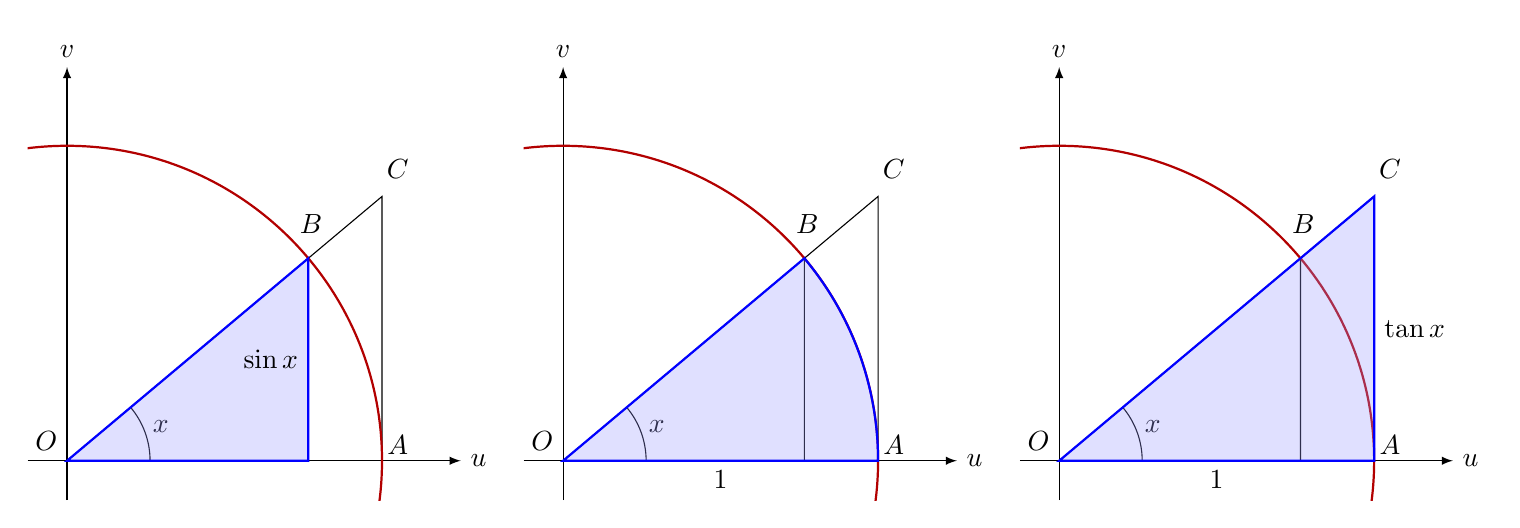
\begin{tikzpicture}[>=latex]
\Base
\filldraw[thick,draw=blue,fill=blue!40,fill opacity=0.3,text opacity=1]
  (O) -- (aux1) -- node[left] {$\sin x$} (aux2)  -- cycle; 

\Base[6.3cm]
\filldraw[thick,draw=blue,fill=blue!40,fill opacity=0.3,text opacity=1]
  (O) -- (aux1) arc (40:0:4) -- node[below] {$1$} cycle; 

\Base[12.6cm]
\filldraw[thick,draw=blue,fill=blue!40,fill opacity=0.3,text opacity=1]
  (O) -- (aux3) -- node[right] {$\tan x$} (aux3|-0,0)  -- node[below] {$1$} cycle; 
\end{tikzpicture}
\vspace{.1cm}
Luego, comparando las areas, $\overset{\triangle}{AOB} <$ \'area sector circular $AOB < \overset{\triangle}{AOC}$.\\
Puesto en valores queda: $\dfrac{|\sin x|}{2} < \dfrac{|x|}{2} < \dfrac{|\tan x|}{2}$ e inmediatamente implica el enunciado.\\

\noindent \textbf{Nota}: La desigualdad $|\sin x| < |x|$ es cierta $\forall x \not = 0$. $|\sin x| \leq 1 < \dfrac{\pi}{2} \leq |x|$\\

\noindent Podemos asegurar tambi\'en que $\displaystyle{\lim_{x\to 0} \sin x} = 0$, pues $0<|x|<\delta \Rightarrow |\sin x| < |x| < \delta < \epsilon$\\

\noindent Tambi\'en es \'util ver que:
\begin{align*}
\cos x &= \cos \left(2\dfrac{x}{2}\right) = \cos\left(\dfrac{x}{2} + \dfrac{x}{2}\right) = \left(\cos \dfrac{x}{2} \cdot \cos \dfrac{x}{2} - \sin \dfrac{x}{2} \cdot \sin \dfrac{x}{2}\right)\\
& = \cos^2 \left(\dfrac{x}{2}\right) - \sin^2 \left(\dfrac{x}{2}\right) = 1 - \sin^2 \left(\dfrac{x}{2}\right) - \sin^2 \left(\dfrac{x}{2}\right) = 1 - 2\cdot \sin^2 \left(\dfrac{x}{2}\right)
\end{align*}
De esta manera podemos concluir que:
$$\lim_{x\to 0}\cos x = \lim_{x\to 0}\left(1 - 2\cdot \sin^2 \left(\dfrac{x}{2}\right)\right) = 1$$

\noindent \textbf{Teorema 8}: Para $a \in \mathbb{R}$:
$$\lim_{x\to a}\sin x = \sin a \ \ \ \ \land \ \ \ \ \lim_{x\to a}\cos x = \cos a$$
\noindent \textbf{Demostraci\'on}: Usando lo anterior m\'as las siguientes formulas:
\begin{itemize}
\item $\displaystyle{\lim_{x\to a}(\sin x) = \lim_{x\to 0} (\sin(x+a)) = \lim_{x\to 0} (\sin x \cdot \cos a + \cos x \cdot \sin a) = 0 \cdot \cos a + 1 \cdot \sin a = \sin a}$
\item $\displaystyle{\lim_{x\to a}(\cos x) = \lim_{x\to 0} (\cos(x+a)) = \lim_{x\to 0} (\cos x \cdot \cos a - \sin x \cdot \sin a) = 1 \cdot \cos a - 0 \cdot \sin a = \cos a}$
\end{itemize}

\noindent \textbf{Corolario 2}: 
\begin{enumerate}
\item Para $a \not = \left(\dfrac{\pi}{2} + k\cdot \pi\right), k \in \mathbb{Z} : \ \ \ \ \displaystyle{\lim_{x\to a} \tan x = \tan a \ \ \ \ \land \ \ \ \ \lim_{x\to a}\sec x = \lim_{x\to a}\dfrac{1}{\cos x} = \dfrac{1}{cos a} = \sec a}$
\item Para $a \not = k\cdot \pi, k \in \mathbb{Z} : \ \ \displaystyle{\lim_{x\to a}\csc x = \lim_{x\to a}\dfrac{1}{\sin x} = \dfrac{1}{\sin a} = \csc a \ \ \land \ \ \lim_{x\to a}\cot x = \lim_{x\to a}\dfrac{\sin x}{\cos x} = \dfrac{\sin a}{\cos a} = \cot a}$\\ \\
\QEDA
\end{enumerate}

\section{El Principio de Intercalaci\'on}
\noindent \textbf{Teorema 9}: \textbf{El Principio de Intercalaci\'on}: Sean $f,g,h$ tres funciones y $a$ un real, tales que en alg\'un entorno reducido $E'(a, \rho)$ se tiene: $g(x) \leq f(x) \leq h(x)$,\\
y adem\'as las funciones $g$ y $h$ tienen l\'imite en $a$ siendo $\displaystyle{\lim_{x\to a} g(x) = \lim_{x\to a} h(x) = l}$,\\
Entonces $f$ tiene l\'imite en el punto $a$ y vale $\displaystyle{\lim_{x\to a} f(x)=l}.$\\
\noindent \textbf{Demostraci\'on}: Tenemos $0<|x-a|<\delta_1 \Rightarrow|g(x)-l| < \epsilon \ \ \land \ \ 0<|x-a|<\delta_2 \Rightarrow |h(x) - l| < \epsilon$\\
Entonces para $\delta = \min\{\rho, \delta_1, \delta_2\}$, y $x$ tal que:
\[0 < |x-a| < \delta \left\{\begin{array}{l}
g(x) \leq f(x) \leq h(x)\\
l - \epsilon < g(x)\\
h(x) < l + \epsilon
\end{array}\right. \Rightarrow (l - \epsilon < f(x) < l + \epsilon) \Rightarrow (|f(x) - l| < \epsilon)\]\\

\noindent \textbf{Proposici\'on 5}: El Principio de Intercalaci\'on es valido si se reemplaza $x\rightarrow a$ por $x\rightarrow a^+$ o $x\rightarrow a^-$.

\noindent \textbf{Proposici\'on 6}: $\displaystyle{\lim_{x \to 0} \dfrac{\sin x}{x} = 1}$\\
\noindent \textbf{Demostraci\'on}: Para $-\dfrac{\pi}{2} < x < \dfrac{\pi}{2}, x \not = 0$, tenemos que $|\sin x| < |x| < |\tan x|$\\
Para los $x$ tales que $0 < x < \dfrac{\pi}{2}$, si dividimos por $\sin x > 0$, tenemos $1 < \dfrac{x}{\sin x} < \dfrac{1}{\cos x}$\\
Para los $x$ tales que $\dfrac{\pi}{2} < x < 0$, si dividimos por $-\sin x > 0$, tenemos $1 < \dfrac{x}{\sin x} < \dfrac{1}{\cos x}$\\
Y como sabemos que $\displaystyle{\lim_{x \to 0} \cos x = 1} \not = 0 \Rightarrow \displaystyle{\lim_{x \to 0} \dfrac{1}{\cos x} = 1}$\\
Utilizando el Teorema del Sandwich, se concluye que $\displaystyle{\lim_{x \to 0} \dfrac{x}{\sin x} = 1 \not = 0}$ y luego $\displaystyle{\lim_{x \to 0} \dfrac{\sin x}{x} = 1}$
\QEDA\\

\noindent Adem\'as, se puede concluir que si $f(x) \not = 0$ en un $E'(a, \rho)$, y $\displaystyle{\lim_{x \to a} f(x) = 0}$ entonces $\displaystyle{\lim_{x \to a} \dfrac{\sin f(x)}{f(x)} = 1}$

\section{Generalizaci\'on del Concepto de L\'imite}
\begin{itemize}
\item Una funci\'on tiene limite $+\infty$ en el punto $a$ si para cualquier $M>0$ existe un $\delta>0$ tal que: $0<|x-a|<\delta \Rightarrow f(x)>M$. Luego, notamos $\displaystyle{\lim_{x \to a} f(x) = +\infty}$
\item Una funci\'on tiene limite $-\infty$ en el punto $a$ si para cualquier $M>0$ existe un $\delta>0$ tal que: $0<|x-a|<\delta \Rightarrow f(x)>-M$ Luego, notamos $\displaystyle{\lim_{x \to a} f(x) = -\infty}$
\end{itemize}

\noindent \textbf{Teorema 10}: \textbf{\'Algebra de L\'imites Infinitos}: Sean $a$ un real, y $f$ y $g$ dos funciones tales que:
\begin{itemize}
\item $\displaystyle{\lim_{x \to a} f(x) = +\infty}$ y $\displaystyle{\lim_{x \to a} g(x) = +\infty}$, entonces $\displaystyle{\lim_{x \to a} (f+g)(x) = +\infty}$
\item $\displaystyle{\lim_{x \to a} f(x) = -\infty}$ y $\displaystyle{\lim_{x \to a} g(x) = -\infty}$, entonces $\displaystyle{\lim_{x \to a} (f+g)(x) = -\infty}$
\item Si $c>0$, $\displaystyle{\lim_{x \to a} f(x) = +\infty}$ y $\displaystyle{\lim_{x \to a} g(x) = -\infty}$, entonces $\displaystyle{\lim_{x \to a} (cf)(x) = +\infty}$ y $\displaystyle{\lim_{x \to a} (cg)(x) = -\infty}$
\item Si $c<0$, $\displaystyle{\lim_{x \to a} f(x) = +\infty}$ y $\displaystyle{\lim_{x \to a} g(x) = -\infty}$, entonces $\displaystyle{\lim_{x \to a} (cf)(x) = -\infty}$ y $\displaystyle{\lim_{x \to a} (cg)(x) = +\infty}$
\item Si $\displaystyle{\lim_{x \to a} f(x) = \pm \infty}$ y $\displaystyle{\lim_{x \to a} g(x) = \pm \infty}$, entonces $\displaystyle{\lim_{x \to a} (f\cdot g)(x) = + \infty}$
\item Si $\displaystyle{\lim_{x \to a} f(x) = \pm \infty}$ y $\displaystyle{\lim_{x \to a} g(x) = \mp \infty}$, entonces $\displaystyle{\lim_{x \to a} (f\cdot g)(x) = - \infty}$
\end{itemize}
\textbf{Demostraciones}
\begin{itemize}
\item $ \left.
\begin{array}{l}
0<|x-a|<\delta' \Rightarrow f(x)>M'\\
0<|x-a|<\delta'' \Rightarrow f(x)>M''
\end{array} \right\} \Rightarrow \delta \leq \min\{\delta', \delta''\}, 0<|x-a|<\delta,
$\\
$(f+g)(x) = f(x)+g(x) < M' + M'' = M \therefore M' = \dfrac{M}{2} \land M'' = \dfrac{M}{2}$ \QEDA

\item $ \left.
\begin{array}{l}
0<|x-a|<\delta' \Rightarrow f(x)>-M'\\
0<|x-a|<\delta'' \Rightarrow f(x)>-M''
\end{array} \right\} \Rightarrow \delta \leq \min\{\delta', \delta''\}, 0<|x-a|<\delta,
$\\
$(f-g)(x) = f(x)-g(x) < -M' + -M'' = M \therefore M' = -\dfrac{M}{2} \land M'' = -\dfrac{M}{2}$ \QEDA

\item $0<|x-a|<\delta_1 \Rightarrow f(x) > M',\ (c\cdot f)(x)=c\cdot f(x) < c\cdot M' = M \therefore M'=\dfrac{M}{c}$\\
\indent $0<|x-a|<\delta_2 \Rightarrow g(x) > -M'',\ (c\cdot g)(x)=c\cdot g(x) < c\cdot -M'' = M \therefore M''= - \dfrac{M}{c}$ \QEDA

\item $0<|x-a|<\delta_1 \Rightarrow f(x) > M',\ (c\cdot f)(x)=c\cdot f(x) < c\cdot M' = -M \therefore M'=-\dfrac{M}{c}$\\
\indent $0<|x-a|<\delta_2 \Rightarrow g(x) > M'',\ (c\cdot g)(x)=c\cdot g(x) < c\cdot M'' = M \therefore M''=\dfrac{M}{c}$

\item $ \left.
\begin{array}{l}
0<|x-a|<\delta' \Rightarrow f(x)>M'\\
0<|x-a|<\delta'' \Rightarrow f(x)>M''
\end{array} \right\} \Rightarrow \delta \leq \min\{\delta', \delta''\}, 0<|x-a|<\delta,
$\\
$(f\cdot g)(x) = f(x)\cdot g(x) < M' \cdot M'' = M \therefore M' = \sqrt{M} \land M'' = \sqrt{M}$ (an\'alogamente el resto)\QEDA
\end{itemize}
\subsection{L\'imites laterales infinitos}
\begin{itemize}
\item Una funci\'on tiene limite $+\infty$ (resp. $-\infty$) por izquierda en el punto $a$, si para $M>0$, $\exists \delta>0$: $$a-\delta<x<a \Rightarrow f(x) > M\ (\text{resp. } f(x)<-M)$$
\item Una funci\'on tiene limite $+\infty$ (resp. $-\infty$) por derecha en el punto $a$, si para $M>0$, $\exists \delta>0$: $$a<x<a+\delta \Rightarrow f(x) > M\ (\text{resp. } f(x)<-M)$$
\end{itemize}

\noindent \textbf{Proposici\'on 7}: \textbf{\'Algebra de L\'imites Laterales Infinitos}: Los resultados del \textit{Teorema 10} son v\'alidos si se reemplazan los s\'imbolos $x\rightarrow a$ por $x\rightarrow a^+$ o $x\rightarrow a^-$.

\section{L\'imites en el Infinito}
\begin{itemize}
\item Una funci\'on $f$ tiene l\'imite $l$ cuando $x \to +\infty$, si $\forall \epsilon > 0$, $\exists H > 0$ :\\ $x > H \Rightarrow |f(x)-l| < \epsilon$ y notamos $\displaystyle{\lim_{x \to +\infty} f(x) = l}$
\item Una funci\'on $f$ tiene l\'imite $l$ cuando $x \to -\infty$, si $\forall \epsilon > 0$, $\exists H > 0$ :\\ $x < -H \Rightarrow |f(x)-l| < \epsilon$ y notamos $\displaystyle{\lim_{x \to -\infty} f(x) = l}$
\end{itemize}
Notamos que si una propiedad se verifica $\forall x > H_1$, y otra propiedad se verifica $\forall x > H_2$, ambas se verifican para $H\geq\max\{H_1,H_2\}$.\\

\noindent \textbf{Proposici\'on 8}: \textbf{\'Algebra de L\'imites en el Infinito}: Los resultados de la secci\'on de \textit{\'Algebra de L\'imites} son v\'alidos si se reemplazan los s\'imbolos $x\to a$ por $x\to +\infty$ o $x\to -\infty$.

\section{L\'imites Infinitos en el Infinito}
\begin{itemize}
\item Una funci\'on $f$ tiene l\'imite $+\infty$ cuando $x\to +\infty$, si $\forall M>0,\ \exists H>0$: ($x>H \Rightarrow f(x)>M$)
\item Una funci\'on $f$ tiene l\'imite $+\infty$ cuando $x\to -\infty$, si $\forall M>0,\ \exists H>0$: ($x<-H \Rightarrow f(x)>M$)
\item Una funci\'on $f$ tiene l\'imite $-\infty$ cuando $x\to +\infty$, si $\forall M>0,\ \exists H>0$: ($x>H \Rightarrow f(x)<-M$)
\item Una funci\'on $f$ tiene l\'imite $-\infty$ cuando $x\to -\infty$, si $\forall M>0,\ \exists H>0$: ($x<-H \Rightarrow f(x)<-M$)
\end{itemize}

\noindent \textbf{Proposici\'on 9}: \textbf{\'Algebra de L\'imites Infinitos en el Infinito}: Los resultados de la secci\'on de \textit{\'Algebra de L\'imites Infinitos} son v\'alidos si se reemplazan los s\'imbolos $x\to a$ por $x\to +\infty$ o $x\to -\infty$.\\


\noindent \textbf{Proposici\'on 10}:
\begin{itemize}
\item $\displaystyle{\lim_{x \to a} f(x) \Rightarrow \pm\infty} \Rightarrow \displaystyle{\lim_{x \to a} \left(\dfrac{1}{f}\right)(x) = 0}$ \\ (Lo mismo ocurre si se reemplaza $x\to a$ por $x\to a^+$, $x\to a^-$, $x\to +\infty$ o $x\to -\infty$).\\
\textbf{Demostraci\'on}: Queremos demostrar que\\ $\left[0<|x-a|<\delta \Rightarrow f(x) > M \right] \Rightarrow \left[0<|x-a|<\delta \Rightarrow \left|\dfrac{1}{f(x)}-0\right|<\epsilon\right]$. \\
Y como $f(x)>M>0 \Rightarrow 0 <\dfrac{1}{f(x)}<\dfrac{1}{M} \Rightarrow \left|\dfrac{1}{f(x)}-0\right| < \dfrac{1}{M}$, consideramos $\dfrac{1}{M} = \epsilon > 0$ \QEDA\\

\item $\displaystyle{\lim_{x \to \pm\infty} f(x) = l} \iff \displaystyle{\lim_{x \to 0^\pm} f\left(\dfrac{1}{x}\right) = l}$ \\ (Lo mismo ocurre si se reemplaza $l$ por $+\infty$ o $-\infty$).\\
\textbf{Demostraci\'on}: Queremos demostrar que\\ $\left[ 0<H<x \Rightarrow |f(x)-l| < \epsilon \right] \iff \left[ 0 < x < 0 + \delta  \Rightarrow \left|f\left(\dfrac{1}{x}\right)-l\right| < \epsilon \right]$\\
Y como $0<H<x \Rightarrow 0<\dfrac{1}{x} < \dfrac{1}{H} \Rightarrow |f(x)-l|<\epsilon$, tomando $\delta = \dfrac{1}{H}$ y haciendo un cambio de variable $x'=x$, tenemos que $0< x' < \delta \Rightarrow \left|f\left(\dfrac{1}{x'}\right)-l\right|<\epsilon$ \QEDA
\end{itemize}

\subsection{L\'imites de Funciones Racionales en el Infinito}
\begin{itemize}
\item Se puede demostrar que si $n \in \mathbb{N}$, entonces $\displaystyle{\lim_{x \to +\infty} x^n = +\infty}$ a trav\'es de la definici\'on formal:\\
$\forall M > 0,\ \exists H>0$ : $x > H > 0 \Rightarrow x^n > M$, luego $x^n > M > 0 \Rightarrow x > H = \sqrt[n]{M} > 0 \Rightarrow x^n > M$\\
Y tenemos que $H = \sqrt[n]{M} > 0$, $x>H=\sqrt[n]{M} \Rightarrow x^n>M$ \QEDA\\

\item Dada la funci\'on polin\'omica $p(x)=x^n+a_{n-1} \cdot x^{n-1}+...+a_1 \cdot x + a_0$, $\displaystyle{\lim_{x \to +\infty} p(x) = +\infty}$. \\
Se empieza sacando factor com\'un $x^n$. Ya esta demostrado que $\displaystyle{\lim_{x \to +\infty} x^n = +\infty}$, y por la $P10$, $\displaystyle{\lim_{x \to +\infty} \dfrac{1}{x^n} = 0}$. Obteniendo as\'i: $\overbrace{x^n}^{\to +\infty}\cdot \overbrace{(1+ \underbrace{a_{n-1} \cdot \dfrac{1}{x}}_{\to 0}+...+\underbrace{a_1 \cdot \dfrac{1}{x^{n-1}}}_{\to 0} + \underbrace{a_0 \cdot \dfrac{1}{x^n}}_{\to 0})}^{\to 1} = +\infty$ \QEDA\\

\item Sean $a_n, b_m \in \mathbb{R} - \{0\}$: \\
$\displaystyle{\lim_{x \to +\infty} \dfrac{a_nx^n + a_{n-1}x^{n-1} + ... + a_1x + a_0}{b_mx^m + b_{m-1}x^{m-1} + ... + b_1x + b_0} = } \left\{\begin{array}{ll}
+\infty &: m<n, a_n\cdot b_m > 0\\
-\infty &: m<n, a_n\cdot b_m < 0\\
\frac{a_n}{b_m} &: m=n\\
0 &: m>n\\
\end{array}\right.
$

\begin{itemize}
\item Si tenemos que $m<n$ y $a_n\cdot b_m > 0 \Rightarrow n-m \in \mathbb{N}$, entonces $\displaystyle{\lim_{x \to +\infty} n^{n-m} = +\infty}$:\\
$\displaystyle{\lim_{x \to +\infty} \underbrace{x^{n-m}}_{\to +\infty} \cdot \underbrace{\dfrac{a_nx^n + a_{n-1}x^{n-1} + ... + a_1x + a_0}{b_mx^m + b_{m-1}x^{m-1} + ... + b_1x + b_0}}_{\to \frac{a_n}{b_m} > 0} = +\infty}$ \QEDA
\item Si $m<n$ y $a_n\cdot b_m < 0 \Rightarrow n-m \in \mathbb{N}$, entonces $\displaystyle{\lim_{x \to +\infty} n^{n-m} = +\infty}$:\\
$\displaystyle{\lim_{x \to +\infty} \underbrace{x^{n-m}}_{\to +\infty} \cdot \underbrace{\dfrac{a_nx^n + a_{n-1}x^{n-1} + ... + a_1x + a_0}{b_mx^m + b_{m-1}x^{m-1} + ... + b_1x + b_0}}_{\to \frac{a_n}{b_m} < 0} = -\infty}$ \QEDA
\item Si $m=n$, entonces $\displaystyle{\lim_{x \to +\infty} n^{n-m} = n^0 = 1}$:\\
$\displaystyle{\lim_{x \to +\infty} \underbrace{x^{n-m}}_{\to +\infty} \cdot \underbrace{\dfrac{a_nx^n + a_{n-1}x^{n-1} + ... + a_1x + a_0}{b_mx^m + b_{m-1}x^{m-1} + ... + b_1x + b_0}}_{\to \frac{a_n}{b_m}} = \dfrac{a_n}{b_m}}$ \QEDA
\item Si $m>n$, $m-n \in \mathbb{N}$, entonces $\displaystyle{\lim_{x \to +\infty} x^{m-n} = +\infty}$ y
$\displaystyle{\lim_{x \to +\infty} x^{n-m} = \lim_{x \to +\infty} \dfrac{1}{x^{m-n}}} = 0$:\\
$\displaystyle{\lim_{x \to +\infty} \underbrace{x^{n-m}}_{\to 0} \cdot \underbrace{\dfrac{a_nx^n + a_{n-1}x^{n-1} + ... + a_1x + a_0}{b_mx^m + b_{m-1}x^{m-1} + ... + b_1x + b_0}}_{\text{ un valor acotado }} = 0}$ \QEDA
\end{itemize}
\end{itemize}

\section{M\'as Algebra de L\'imites}
\textbf{Teorema}: Sea $a\in\mathbb{R}$,$f$ y $g$ funciones tales que: $\displaystyle{\lim_{x \to a^+} f(x) = L}\ \land \ \displaystyle{\lim_{x \to a^+} g(x) = +\infty}\ \land\ \displaystyle{\lim_{x \to a^+} h(x) = -\infty} $ 


$$ \displaystyle{\lim_{x \to a^+} (f+x)(x) = +\infty}$$
$$ \displaystyle{\lim_{x \to a^+} (f+h)(x) = -\infty}$$
$$ \lim_{x \to a^+} (fg)(x) = \left\{\begin{array}{ll} +\infty &, L>0\\ -\infty &, L<0 \end{array}\right.$$
Se puede reemplazar $x\to a^+$ por $x\to a^-$, $x\to +\infty$ o $x\to -\infty$.

\section{As\'intotas}
\noindent Se dice que la recta vertical $x=a$ es una \textbf{asíntota vertical} de la función $f$ en el punto $a$ si se verifica por lo menos uno de estos cuatro límites:
\begin{multicols}{4}
$\displaystyle{\lim_{x \to a^+} f(x) = +\infty}$\\
$\displaystyle{\lim_{x \to a^+} f(x) = -\infty}$\\
$\displaystyle{\lim_{x \to a^-} f(x) = +\infty}$\\
$\displaystyle{\lim_{x \to a^-} f(x) = -\infty}$
\end{multicols}

\noindent Se dice que la recta horizontal $y=b$ es una \textbf{asíntota horizontal} de la función $f$ si se verifica por lo menos uno de estos dos límites:
\begin{multicols}{4}
\ \\
$\displaystyle{\lim_{x \to +\infty} f(x) = b}$\\
$\displaystyle{\lim_{x \to -\infty} f(x) = b}$\\
\ 
\end{multicols}

\noindent Se dice que la recta $y=mx+b$, con $m \not = 0$, es una \textbf{asíntota oblicua} de la función $f$ si se verifica por lo menos uno de estos dos límites:
\begin{multicols}{2}
$\displaystyle{\lim_{x \to +\infty} (f(x)-(mx+b)) = 0}$\\
$\displaystyle{\lim_{x \to -\infty} (f(x)-(mx+b)) = 0}$
\end{multicols}

\section{L\'imites Indeterminados}
\begin{itemize}
\item Cociente de dos funciones con l\'imite cero: $\dfrac{0}{0}$
\item Cociente de dos funciones con l\'imite infinito: $\dfrac{\infty}{\infty}$
\item Producto de un l\'imite cero por uno infinito: $0\cdot \infty$
\item Suma de dos infinitos de distinto signo: $\pm \infty + \mp \infty$
\end{itemize}
Cuando se tiene una indeterminaci\'on del l\'imite, el l\'imite puede ser un n\'umero real o incluso $\pm \infty$, y hay que realizar simplificaciones o reemplazos para poder calcularlo.\\
\textbf{Nota}: Si tenemos $g(x)$ definida en un entorno reducido del punto $a$, donde no se anula y que tiende a $0$ en dicho punto, entonces $\dfrac{0}{g(x)} = 0$, y por Caracter Local del Limite, $\displaystyle{\lim_{x \to a} \dfrac{0}{g(x)} = 0}$\\
\textbf{Nota}: Las consideraciones hechas para el c\'alculo de l\'imites puntuales valen para los l\'imites en el infinito y para el c\'alculo de l\'imites laterales, con los mismos casos de indeterminaci\'on.

\section{Definici\'on de Continuidad}
Sean $f$ una funci\'on y $a$ un n\'umero real, entonces se dice que: $f$ es continua en $a$ $\iff$
\begin{enumerate}
\item Existe el valor $f(a)$,
\item Existe el valor $\displaystyle{\lim_{x \to a} f(x)}$ y es finito,
\item $\displaystyle{\lim_{x \to a} f(x) = f(a)}$.
\end{enumerate}
Definiendo usando entornos de $a$ y $f(a)$, $$\text{$f$ es continua en $a$ } \iff \forall\ \epsilon > 0,\ \exists \delta > 0 :\ |x-a|<\delta \Rightarrow |f(x)-f(a)| < \epsilon$$
Difiriendo de la definici\'on de l\'imite al reemplazar $l$ por $f(a)$ y la condici\'on se debe verificar en el entorno completo, ya que $f$ debe estar definida en $a$ (en dicho punto vale $\forall\ \epsilon>0$, ya que $|f(a)-f(a)| = 0 < \epsilon$).

\subsection{Continuidad Lateral}
Una funci\'on $f$ se dice continua por izquierda (resp. derecha) en el punto $a$, si existe el valor de $f(a)$, el valor del l\'mite lateral por izquierda (resp. derecha) y ambos coinciden.
\subsection{Funciones Continuas}
Una funci\'on se dice que es continua si es continua en todos los puntos de su dominio. Entre ellas:
\begin{itemize}
\item La funci\'on lineal $f(x)=m\cdot x + h$.
\item Los polinomios y las funciones racionales.
\item Las funciones seno y coseno, y las dem\'as funciones trigonom\'etricas.
\item La funcion valor absoluto $f(x)=|x|$.
\end{itemize}

\section{Discontinuidades}
\subsection{Discontinuidad Evitable}
Sucede cuando existe el l\'imite finito de la funci\'on en un punto, pero no coincide con el valor de la funci\'on en dicho punto (pudiendo incluso no estar definido).
\subsection{Discontinuidad Inevitable de Salto Finito}
Sucede cuando una funci\'on posee ambos l\'imites laterales finitos, pero no coinciden. La distancia entre ambos l\'imites se la denomina discontinuidad del salto.
\subsection{Discontinuidad Inevitable de Salto Infinito}
Sucede si al menos uno de los dos l\'imites laterales en un punto es infinito y el otro existe, siendo el segundo finito o infinito.
\subsection{Discontinuidades Esenciales}
Sucede si alli la discontinuidad no es evitable, ni de salto finito o infinito. En el punto no existe uno de los l\'imites laterales, finito o infinito.\\
Ejemplos: 
\begin{itemize}
\item $f(x)=\left\{\begin{array}{ll} 1 & \text{ si } x \in \mathbb{Q} \\ 0 & \text{ si } x \in \mathbb{R - Q}\end{array}\right.$ \\ Es discontinua en todo n\'umero real. Dado $\epsilon = \frac{1}{2}$, y $a$ racional, en cualquier entorno $E(a,\delta)$ existen irracionales para los cuales $|f(x)-f(a) = |0-1| = 1 > \frac{1}{2} = \epsilon$. An\'alogamente para los $b$ irracionales, en $E(b,\delta)$ existen racionales en los que $|f(x)-f(a)| = |1-0| = 1 > \frac{1}{2} = \epsilon$. Como en ning\'un punto la funci\'on es continua, tiene discontinuidades esenciales en todos los puntos.
\item $f(x)=\sin\left(\dfrac{1}{x}\right)$. Tiene una discontinuidad esencial en $0$, ya que a medida que se acerca a $0$, los valores fluctuan entre -1 y 1, sin tender a ning\'un valor. Es continua en todo punto distinto de 0.
\item $f(x)=x\cdot\sin\left(\dfrac{1}{x}\right)$. Es continua en todo $\mathbb{R}$. Es continua en 0 por el T6\footnote{$\displaystyle{\lim_{x\to a}f(x) = 0}$ y $g$ est\'a acotada en un entorno reducido $E'(a,\rho)$, entonces $\displaystyle{\lim_{x\to a}(fg)(x) = 0}$}, en el resto por composici\'on de funciones continuas.
\end{itemize}

\section{Teoremas de Funciones Continuas}
\textbf{Proposici\'on 11}: Sea $f$ una funci\'on continua en $a$, entonces existe un entorno de $a$ en el cual $f$ est\'a acotada. Es decir, existen $\delta > 0$, $M > 0$ : $x \in E(a, \delta) \Rightarrow |f(x)| \leq M$\\
\noindent \textbf{Proposici\'on 12}: Sea $f$ una funci\'on continua en $a$ y $k$ un n\'umero real tal que $f(a) > k$ (resp. $f(a) < k$), entonces existe un entorno de $a$ en el cual $f$ asume valores todos mayores (resp. menores) a $k$, es decir, existe $\delta > 0$ : $x \in E(a,\delta) \Rightarrow f(x) > k$ (resp. $f(x) < k$).\\
\noindent \textbf{Corolario 3}: \textbf{Principio de Conservaci\'on del Signo}: Sea $f$ continua en $a$, tal que $f(a)>0$ (resp. $f(a)<0$), entonces existe un entorno de $a$ en el cual la funci\'on se mantiene positiva (resp. negativa).\\
\noindent \textbf{Corolario 4}: Sea $f$ una funci\'on continua en $a$ tal que, en cualquier entorno de $a$ la funci\'on asume tanto valores positivos como negativos, entonces $f(a)=0$. Se demuestra por el absurdo, ya que si suponemos $f(a)>0$ entonces tenemos un entorno de $a$ donde $f$ es siempre positiva, contradiciendo la hipotesis, luego $f(a)\leq 0$. Analogamente suponemos $f(a)<0$, y llegamos a que $f(a)\geq 0$ $\Rightarrow f(a)=0$.\\

\noindent \textbf{Teorema 11}: \textbf{\'Algebra de Funciones Continuas}: Sean $f$ y $g$ funciones continuas en $a$, entonces son continuas en $a$ las funciones $f \pm g$, $c \cdot f (c \in \mathbb{R})$, $f \cdot g$ y $\frac{f}{g}\ (g(a) \not = 0)$.\\
\noindent \textbf{Demostraci\'on}: Sabemos que existen $f(a)$ y $g(a)$, luego existe $(f+g)(a) = f(a) + g(a)$. Ademas existen los l\'imites de $f$ y $g$ en $a$, y vale $\displaystyle{\lim_{x \to a} (f+g)(x) = \lim_{x \to a} f(x) + \lim_{x \to a} g(x) = f(a) + g(a) = (f+g)(a)}$. \QEDA\\
\noindent \textbf{Teorema 12}: \textbf{L\'imite de la Funci\'on Compuesta}: Sean $f$ y $g$ dos funciones tales que $Rec(g) \subset Dom(f)$. Si existe el l\'imite $\displaystyle{\lim_{x \to a} g(x) = l}$ y que $f$ es continua en $l$, entonces existe $\displaystyle{\lim_{x \to a} (f\circ g)(x) = f(l)}$.\\
\textbf{Demostraci\'on}: Queremos llegar a que $0<|x-a|<\delta \Rightarrow |(f \circ g)(x) - f(l)| < \epsilon$. Partiendo con ese $\epsilon$, sabemos que existe $\rho > 0$ para el cual $|z-l| < \rho \Rightarrow |f(z)-f(l)| < \epsilon$. Y como $0 < |x-a| < \delta \Rightarrow |g(x) - l| < \rho$, combinando las expresiones llegamos a que: $$0 < |x-a| < \delta \Rightarrow |g(x)-l| < \rho \Rightarrow |f(g(x)) - f(l)| < \epsilon $$ \QEDA\\
\noindent \textbf{Corolario 5}: \textbf{Continuidad de la Funci\'on Compuesta}: Sea $g$ continua en $a$ y $f$ continua en $g(a)$, entonces $(f\circ g)(a)$ es continua en $a$.

\section{Ceros de Funciones Continuas y Teorema de Bolzano}
\noindent \textbf{Teorema 13}: \textbf{Teorema de Bolzano}: Sea $f$ una funci\'on continua en el intervalo $[a,b]$ : $f(a)\cdot f(b) < 0$ (i.e tienen distino signo), entonces existe $\xi \in (a,b)$ donde $f(\xi) = 0$.\\
\indent Recordando el teorema de conservaci\'on de signo de las funciones continuas, que se demuestra m\'as adelante, Sea $f$ continua en $c$, y supongamos que $f(c)\not = 0$, existe entonces un intervalo $(c-\rho, c+\rho)$ en el que $f$ tiene el mismo signo que $f(x)$.\\
\textbf{Demostraci\'on del Teorema de Bolzano}: Supongase $f(a)<0$ y $f(b)>0$. Sea $S$ el conjunto de todos los puntos del intervalo $[a,b]$ para los cuales $f(x)\leq 0$. Hay al menos un punto, puesto que $f(a) < 0$. Luego, $S$ es un conjunto no vacio y est\'a acotado superiormente, puesto que todos los valores est\'an en $[a,b]$, luego tiene un supremo, llam\'emoslo $c$. Y se demostrar\'a que $f(c)=0$.\\
\indent Como sabemos por tricotom\'ia que solo hay 3 posibilidades, $f(c) > 0\ \underline{\lor}\ f(c) < 0\ \underline{\lor}\ f(x) = 0$.\\
\indent Comenzamos suponiendo que $f(x)>0$, luego existe un intervalo $(c-\delta, c+\delta)$, o $(c-\delta, c)$ si $c=b$, en donde si $x$ est\'a en ese intervalo $f(x)$ es positivo. Y como ning\'un punto mayor que $c-\delta$ puede pertenecer al conjunto $S$ (puesto que su imagen es positiva), entonces $c-\delta$ es una cota superior de $S$. Lo cual contradice que $c$ es supremo del conjunto.\\
\indent Suponiendo que $f(c) < 0$, luego existe un intervalo $c-\delta,c+\delta$ (o $(c, c+\delta$ si $a=c$) en donde si $x$ pertenece a dicho intervalo, entonces su imagen es negativa. Pero entonces existe $x > c$ tal que su imagen es menor que cero, entonces $x$ deberia pertenecer al conjunto, y contradice que $c$ sea el supremo del mismo.\\ 
\indent Luego, solo queda la posibilidad de que $f(c)=0$ y queda demostrado el Teorema de Bolzano. \QEDA\\

\noindent \textbf{M\'etodo de Bisecci\'on}: Dada una funci\'on $f$ continua en un intervalo, que asume valores de diferente signo en los extremos, sucesivamente se calculan los valores de dos sucesiones $a_n$ y $b_n$ que convergen a un cero de la funci\'on. Conocidos $a_n$ y $b_n$, se calcula el valor del punto medio $c_{n+1} = \dfrac{a_n+b_n}{2}$ y se tendr\'a que el valor $c_{n+1}$ aproxima al valor $\xi$ de un cero, con cota $|c_{n+1} - \xi| \leq \dfrac{b-a}{2^{n+1}}$. Es decir, dada una tolerancia $\epsilon$, buscamos $n$ para el cual $\dfrac{b-a}{2^{n+1}} < \epsilon$, encontrando un valor $c_{n+1}$ a menos de una distancia $\epsilon$ de $\xi$.\\

\textbf{Nota}: El cero de $f$ puede no ser \'unico, y si se utilizan otros puntos $a$ y $b$, quizas se encuentran ceros diferentes.\\

\noindent \textbf{Teorema 14}: \textbf{Propiedad de los Valores Intermedios}: Sea $f$ una funci\'on continua en $[a,b]$, donde $f(a) \not = f(b)$ y $k$ un valor comprendido estrictamente entre $f(a)$ y $f(b)$, entonces existe un punto $\xi \in (a,b)$ para el cual resulta $f(\xi)=k$\\
\noindent \textbf{Demostraci\'on}: Supongamos $f(a)<f(b)$ (si no sucede, es an\'alogo), entonces $f(a)<k<f(b)$. Luego definimos la funci\'on $g(x) = f(x)-k$, y tenemos que $g$ es continua en $[a,b]$ por ser resta de funciones continuas, $g(a)<0$ y $g(b)>0$. Y al satisfacer las hip\'otesis del Teorema de Bolzano, entonces existe un valor $\xi \in (a,b)$ para el cual $0=g(\xi) = f(\xi)-k \therefore f(\xi)=k$

\textbf{Nota}: Dada la funci\'on potencia $f(x)=x^m$, sabemos que es continua. Con PVI y la Propiedad Arquimediana se puede demostrar que todo n\'umero real (real positivo, si $m$ par) es imagen de alg\'un otro. Por ejemplo, $m=2$ se empieza con que dado $y\in \mathbb{R}^+_0$ $0<y<1 \Rightarrow \exists 0<x<1\ :\ f(x)=y$. Luego si $1\leq y$ por Propiedad Arquimediana se sabe que existe $y<n$, luego $f(1)=1\leq y<n\leq n^2 = f(n)$ y aplicando PVI existe $1\leq x < n$ tal que $f(x)=y$.

\section{Continuidad de la Funci\'on Inversa}
Sabemos que una funci\'on biyectiva admite una funci\'on inversa, y que la misma tambien es biyectiva. Adem\'as, sabemos que es creciente si $\forall x_1, x_2 \in A$, $x_1 < x_2 \Rightarrow f(x_1) < f(x_2)$\\

\noindent \textbf{Teorema 15}: \textbf{Continuidad de la Funci\'on Inversa}: Si $f$ es creciente y continua en un intervalo $[a,b]$, entonces:
\begin{enumerate}
\item Existe la funci\'on inversa $f^{-1}$ definida sobre el intervalo $[f(a),f(b)]$
\item $f^{-1}$ es creciente en $[f(a),f(b)]$
\item $f^{-1}$ es continua en $[f(a),f(b)]$
\end{enumerate}
\textbf{Demostraci\'on}: 
\begin{enumerate}
\item $f$ creciente implica $f$ inyectiva o biyectiva restringiendo el dominio. Luego $Rec(f)=[f(a),f(b)]$, por PVI, como $f$ es continua sobre $[a,b]$, podemos asegurar que dado un $z\in[f(a),f(b)]$, existe un $c\in[a,b])$ tal que $f(c) = z$. Luego $f$ admite inversa, y el domino es $[f(a),f(b)]$.
\item Sean $y_1, y_2$ dos puntos cualesquiera de $[f(a),f(b)]$, y sean $x_1, x_2 \in [a,b]$ tales que $f(x_1)=y_1$ y $f(x_2)=y_2$, para mostrar que $f^{-1}$ es creciente, habr\'a que ver que $y_1<y_2 \Rightarrow f^{-1}(y_1) < f^{-1}(y_2)$:
\begin{align*}
\bigg( y_1<y_2 \Rightarrow f^{-1}(y_1) < f^{-1}(y_2) \bigg) & \iff \bigg( f(x_1)<f(x_2) \Rightarrow f^{-1}(f(x_1)) < f^{-1}(f(x_2)) \bigg)\\
& \iff \bigg( f(x_1)<f(x_2) \Rightarrow x_1 <x_2 \bigg)
\end{align*}
Si $x_1 > x_2$ con $f(x_1)<f(x_2)$, contradice que es creciente. Si $x_1 = x_2$ con $f(x_1)<f(x_2)$, contradice que es funci\'on. Ergo, $f^{-1}$ es creciente mon\'otona sobre $[f(a),f(b)]$.
\item DEMOSTRAR!!!!!!!! TO DO
\end{enumerate}

\noindent \textbf{Teorema 16}: Si $f$ es decreciente y continua en un intervalo $[a,b]$, entonces:
\begin{enumerate}
\item Existe la funci\'on inversa $f^{-1}$ definida sobre el intervalo $[f(a),f(b)]$
\item $f^{-1}$ es decreciente en $[f(a),f(b)]$
\item $f^{-1}$ es continua en $[f(a),f(b)]$
\end{enumerate}

\section{Valores Extremos y Teoremas de Weierstrass}
Sea $f$ una funci\'on definida sobre un conjunto $A$, diremos que:
\begin{itemize}
\item el valor $M$ es el \textbf{m\'aximo} de $f$ en $A$ si existe un n\'umero $x^* \in A$ : $M = f(x^*) \geq f(x),\ \forall x \in A$.
\item el valor $m$ es el \textbf{m\'aximo} de $f$ en $A$ si existe un n\'umero $x^* \in A$ : $Mm= f(x^*) \leq f(x),\ \forall x \in A$.
\end{itemize}
Luego notamos $\ \ \ \ M = \displaystyle{\max_{x\in A} f(x)} \ \ \ \ $ y $\ \ \ \ m = \displaystyle{\min_{x\in A} f(x)}$\\

\textbf{Nota}: $\displaystyle{\max_{x\in A} f(x)}$ = $\displaystyle{-\min_{x\in A} (-f)(x)} \ \ \ \ $ y $\ \ \ \ \displaystyle{\min_{x\in A} f(x)}$ = $\displaystyle{-\max_{x\in A} (-f)(x)}$

\noindent \textbf{Teorema 17}: \textbf{Primer Teorema de Weierstrass}: Si $f$ es una funci\'on continua en un intervalo $[a,b]$, entonces $f$ est\'a acotada en dicho intervalo.\\

\noindent \textbf{Teorema 18}: \textbf{Segundo Teorema de Weierstrass}: Si $f$ es una funci\'on continua en un intervalo $[a,b]$, entonces $f$ alcanza sus valores m\'aximo y m\'inimo en $[a,b]$.\\
\textbf{Demostraci\'on}: Por W1, $f$ est\'a acotada en $[a,b]$, es decir, $\exists M$ : $f(x)\leq M\ \forall x \in [a,b]$.\\ Luego $M$ puede pertenecer o no al $Rec(f)$. \\ 
Suponiendo que no pertenece, es decir, $f(x)<M, \forall x \in [a,b]$, tenemos que $M-f(x)>0,\ \forall x \in [a,b]$. Luego queda bien definida la funci\'on $g(x)=\dfrac{1}{M-f(x)}$ (la cual es continua por ser la rec\'iproca de una funci\'on continua). Nuevamente por W1, $g$ est\'a acotada en el intervalo $[a,b]$. Por lo tanto, existe $M' > 0$ : $g(x) < M',\ \forall x \in [a,b]$. En consecuencia se tiene que:
$$0 < g(x) < M' \Rightarrow 0 < \dfrac{1}{M-f(x)} < M' \Rightarrow 0 < \dfrac{1}{M'} < M - f(x) \Rightarrow f(x) < M-\dfrac{1}{M'} < M$$
Lo cual quiere decir que $f$ admite una cota superior estrictamente menor que $M$, asumido como supremo.\\
\indent Entonces $M$ tiene que pertenecer al $Rec(f)$, luego existe $x^* \in Dom(f)$ : $f(x^*)=M$ y la existencia del m\'aximo est\'a probada.\\

\noindent \textbf{Teorema 19}: \textbf{Teorema de los Valores Intermedios}: Sea $f$ una funci\'on definida en un intervalo cerrado y acotado $[a,b]$, y supongamos que $f$ es continua en $[a,b]$, con $m$ y $M$ sus respectivos valores m\'inimo y m\'aximo absolutos. Entonces, $f$ alcanza todos los valores entre $m$ y $M$. Es decir, $Rec(f) = [m,M]$
\end{document}